\documentclass[letter, 11pt]{article}
%% ================================
%% Packages =======================
\usepackage[utf8]{inputenc}      %%
\usepackage[T1]{fontenc}         %%
\usepackage{lmodern}             %%
\usepackage[spanish]{babel}      %%
\decimalpoint                    %%
\usepackage{fullpage}            %%
\usepackage{fancyhdr}            %%
\usepackage{graphicx}            %%
\usepackage{amsmath}             %%
\usepackage{amssymb}             %%
\usepackage{color}               %%
\usepackage{mdframed}            %%
\usepackage[colorlinks]{hyperref}%%
%% ================================
%% ================================

%% ================================
%% Page size/borders config =======
\setlength{\oddsidemargin}{0in}  %%
\setlength{\evensidemargin}{0in} %%
\setlength{\marginparwidth}{0in} %%
\setlength{\marginparsep}{0in}   %%
\setlength{\voffset}{-0.5in}     %%
\setlength{\hoffset}{0in}        %%
\setlength{\topmargin}{0in}      %%
\setlength{\headheight}{54pt}    %%
\setlength{\headsep}{1em}        %%
\setlength{\textheight}{8.5in}   %%
\setlength{\footskip}{0.5in}     %%
%% ================================
%% ================================

%% =============================================================
%% Headers setup, environments, colors, etc.
%%
%% Header ------------------------------------------------------
\fancypagestyle{firstpage}
{
  \fancyhf{}
  \lhead{
\includegraphics[height=4.5em]{LogoDFI.jpg}}
  \rhead{FI3104-1 \semestre\\
         Métodos Numéricos para la Ciencia e Ingeniería}
  \fancyfoot[C]{\thepage}
}

\pagestyle{plain}
\fancyhf{}
\fancyfoot[C]{\thepage}
%% -------------------------------------------------------------
%% Environments -------------------------------------------------
\newmdenv[
  linecolor=gray,
  fontcolor=gray,
  linewidth=0.2em,
  topline=false,
  bottomline=false,
  rightline=false,
  skipabove=\topsep
  skipbelow=\topsep,
]{ayuda}
%% -------------------------------------------------------------
%% Colors ------------------------------------------------------
\definecolor{gray}{rgb}{0.5, 0.5, 0.5}
%% -------------------------------------------------------------
%% Aliases ------------------------------------------------------
\newcommand{\scipy}{\texttt{scipy}}
%% -------------------------------------------------------------
%% =============================================================

%% =============================================================================
%% CONFIGURACION DEL DOCUMENTO =================================================
%% Llenar con la información pertinente al curso y la tarea
%%
\newcommand{\fechaentrega}{15/09/2019 23:59 hrs}
\newcommand{\semestre}{2019B}
%% =============================================================================
%% =============================================================================


\begin{document}
\thispagestyle{firstpage}

\begin{center}
  {\uppercase{\LARGE \bf Informe Tarea 4}}
\end{center}

\noindent{\Large Tomás Rojas C.}\\
\noindent{\Large RUT:19.688.339-8}\\
\noindent{\Large Github: @tomasrojasc}\\
\noindent{\Large Fecha de entrega: \fechaentrega}

%% =============================================================================
%% ============================================================================

\section{Introducción.}

En este informe se resuelve un problema circuital con dos técnicas distintas, la idea es ver cómo cambian los tiempo de ejecución según el método utilizado. Como nota, el problema que se resuelve en este informe es la implementación real del circuitodel enunciado, con los valores reales, vale decir, sumas de corrientes planteadas en el enunciado

\section{Resolución del problema.}


Lo primero que hay que hacer cuando nos enfrentamos a un problema de este tipo, es plantear las ecuaciones circuitales, estas están dadas por las leyes de Kirchoff, en este caso se va a usar la \emph{ley de voltajes de Kirchoff} utilizando el método de mallas. Esta leyParte de la base que los campos eléctricos presentes en un circuito concentrado son conservativos, por lo que la suma de sus potenciales en un circuito cerrado es siempre cero. Para poder utilizar esta ley adecuadamente, nos vamos a valer de la ley de Ohm que para resistencias puras, nos da la siguiente relación corriente-voltaje:

\begin{equation*}
  V=RI
\end{equation*}

Donde $V$ es el voltaje, $R$ una resistencia y $I$ la corriente que pasa a través de esa resistencia.

Usando los métodos anteriormente descritos y teniendo en cuenta el circuito del enunciado, obtenemos el siguiente sistema de ecuaciones:
\begin{equation*}
\begin{align}
  V&=2RI_1+RI_4\\
  V&=2RI_2+RI_4-RI_5\\
  V&=2RI_3-RI_5\\
  V_1&=RI_1+RI_2+(2R+R_2)I_4+R_2I_6\\
  V_1&=-RI_2-RI_3+(2R+R_2)I_5+R_2I_7\\
  V_1&=R_2I_4+(R+R_2)I_6-RI_8\\
  V_1&=R_2I_5+(R+R_2)I_7+RI_8\\
  V_2&=-RI_6+RI_7+2RI_8
\end{align}
\end{equation*}


Que matricialmente se ve de la siguiente manera:

\begin{equation*}
\begin{bmatrix}
2R & 0  & 0  & R      &   0        &   0       &   0       &   0 \\
0  & 2R & 0  & R      &   -R       &   0       &   0       &   0 \\
0  & 0  & 2R & 0      &   -R       &   0       &   0       &   0 \\
R  & R  & 0  & 2R+R_2 &   0        &   R_2     &   0       &   0 \\
0  & -R & -R & 0      &   2R+R_2   &   0       &   R_2     &   0 \\
0  & 0  & 0  & R_2    &   0        &   R+R_2   &   0       &   -R \\
0  & 0  & 0  & 0      &   R_2      &   0       &   R+R_2   &   R \\
0  & 0  & 0  & 0      &   0        &   -R      &   R       &   2R
\end{bmatrix}
\cdot
\begin{bmatrix}
I_1\\
I_2\\
I_3\\
I_4\\
I_5\\
I_6\\
I_7\\
I_8
\end{bmatrix}
=
\begin{bmatrix}
V\\
V\\
V\\
V_1\\
V_1\\
V_1\\
V_1\\
V_2
\end{bmatrix}
\end{equation*}




Dados los siguientes valores: $R=4[\Omega]$, $R_2=3[\Omega]$, $V=20[V]$ y $V_1=30[V]$. Se nos pide encontrar el valor máximo de $V_2$ que garantiza que por ninguna resistencia pasen más de 20 amperes. Lo primero que hay que notar, es que las corrientes que pasan por las resistencias son combinaciones lineales de las corrientes etiquetadas del 1 al 8. Las corrientes que pasan por cada resistencia está dada por la siguiente lista:


\begin{equation}
  \text{Corrientes}=\{I_1,I_1+I_4,I_4+I_2,I_2-I_5,I_5-I_3,I_3,I_4+I_6,I_5+I_7,I_6-I_8,I_8+I_7\}
\end{equation}


Como es una combinación lineal de las corrientes del sistema, podemos crear una transformación lineal que tenga por salida un vector con todas las corrientes que pasan por las resistencias, de esta manera será más fácil trabajar en el código.



\begin{equation*}
\begin{bmatrix}
1 & 0 &  0  & 0 & 0  & 0 & 0 & 0 \\
1 & 0 &  0  & 1 & 0  & 0 & 0 & 0 \\
0 & 1 &  0  & 1 & 0  & 0 & 0 & 0 \\
0 & 1 &  0  & 0 & -1 & 0 & 0 & 0 \\
0 & 0 &  -1 & 0 & 1  & 0 & 0 & 0 \\
0 & 0 &  1  & 0 & 0  & 0 & 0 & 0 \\
0 & 0 &  0  & 1 & 0  & 1 & 0 & 0 \\
0 & 0 &  0  & 0 & 1  & 0 & 1 & 0 \\
0 & 0 &  0  & 0 & 0  & 1 & 0 & -1 \\
0 & 0 &  0  & 0 & 0  & 0 & 1 & 1
\end{bmatrix}
\cdot
\begin{bmatrix}
I_1\\
I_2\\
I_3\\
I_4\\
I_5\\
I_6\\
I_7\\
I_8
\end{bmatrix}
=
\vec{I}_\text{máximas}
\end{equation*}


Aí solo tenemos que sacar el módulo de cada componente en numpy, función que viene integrada y después solo hay que asegurarse que cada componente sea menor a 20 amperes.


\section{Resultados.}

\subsection{Solución con Cramer.}



Para solucionar este problema, primero usamos el método de Cramer, que fue implementado desde cero. La idea es que forme parte de una gran función en donde entre un voltaje candidato a ser el máximo pedido, y entregue una salida que es la corriente máxima que pasa por una resistencia cualquiera, que en el caso ideal, es cero ya que se resta 20 para que el 0 esté en la salida 20.

Lo primero fue usar el método de Cramer con bisección, lo que no tuvo éxito en el intervalo sugerido en el enunciado, por lo que para asegurarnos, se hizo una función que ve si es viable resolver el método por bisección en un intervalo dado, la respuesta fue negativa. Además se hizo un gráfico que barre un área mayor con tal de ver cómo se comporta la función objetivo.


\begin{figure*}[h]
 \centering
 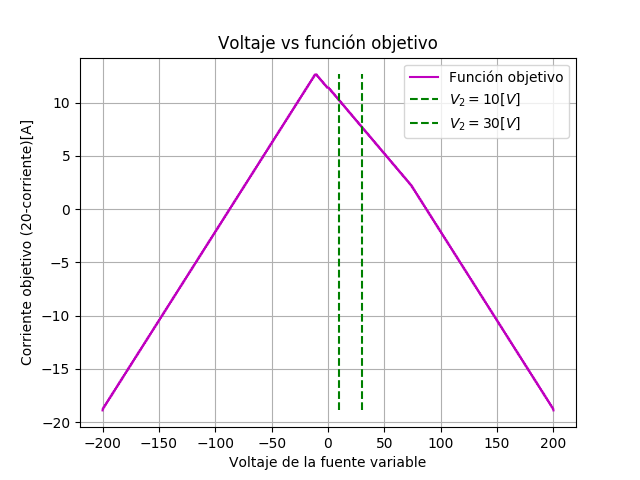
\includegraphics[width=0.8\textwidth]{./img1.png}
 \caption{Gráfico de la función objetivo, método de Cramer.}
\end{figure*}

Podemos notar que claramente no hay solución en en intervalo propuesto, pero sí hay solución en dos puntos. Para encontrar las soluciones podemos usar un algoritmo de bisección con extremos [-100,-50] y [50,100] De esta manera vamos a encontrar dos soluciones para el problema.


Con el método de Cramer, en promedio se demoró $0.014 [s]$

Vemos que en el gráfico hecho con el método de Cramer, hay una discontinuidad extraña, se revisó el código repetidas veces sin poder encontrar su causa. en cualquier caso, la solución es bastante cercana a la solución real que se obtuvo usando el método de descomposición PLU

\subsection{Descomposición PLU.}

Acá usamos una descomposición PLU con la librería de álgebra lineal de scipy. Podemos corroborar con este método, que la solución real no estaba en el rango sugerido.

\begin{figure*}[h]
 \centering
 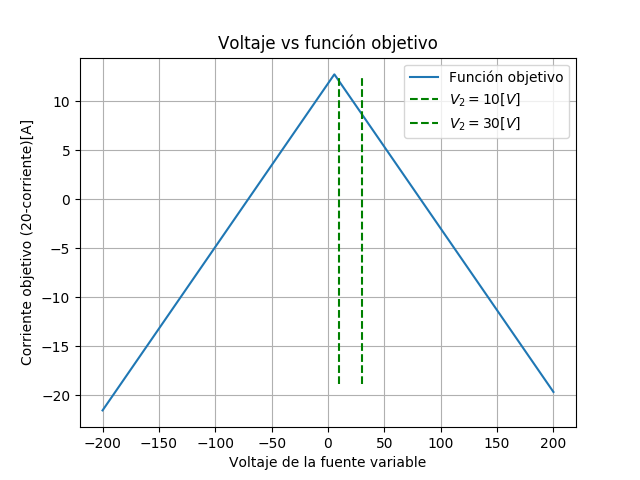
\includegraphics[width=0.8\textwidth]{./img2.png}
 \caption{Gráfico de la función objetivo, método descomposición PLU.}
\end{figure*}


La descomposición PLU, descompone la matriz M en dos matrices triangulares, una inferior y otra superior, y una matriz de permutación.

Este método tomó en promedio $0.0014 [s]$ lo que es un orden de magnitud entero de diferencia con respecto al método de Cramer. por lo que es una diferencia considerable.


\section{Conclusión y discusión.}

los resultados fueron los siguientes:

Cramer:\\

Con el método de Cramer obtuvimos dos soluciones, la primera -87 y la segunda 87

PLU:\\
Con el método de descomposición PLU obtuvimos dos soluciones, la primera -70 y la segunda 82


Claramente estas soluciones difieren, y para ser sinceros, en el código no se ve nada extraño que pueda ser la causa. Por otro lado, para el problema original de evitar que cada corriente pase 20 amperes las soluciones fueron:


Cramer:\\

Con el método de Cramer obtuvimos dos soluciones, la primera -87 y la segunda 87

PLU:\\
Con el método de descomposición PLU obtuvimos dos soluciones, la primera -70 y la segunda 82

Para corroborar estos resultados, se usó el software gratis LTSpice, donde se pudo corroborar que en efecto las soluciones dadas por el método de Cramer, son las correctas. Por lo que seguramente al usar las librerías de scipy, hubo algún error al momento de usarlas todas para obtener la respuesta y seguramente se usaron de mala manera.

Acá podemos ver que LTSpice corrobora lo encontrado por el método de Cramer.


\begin{figure*}[h]
 \centering
 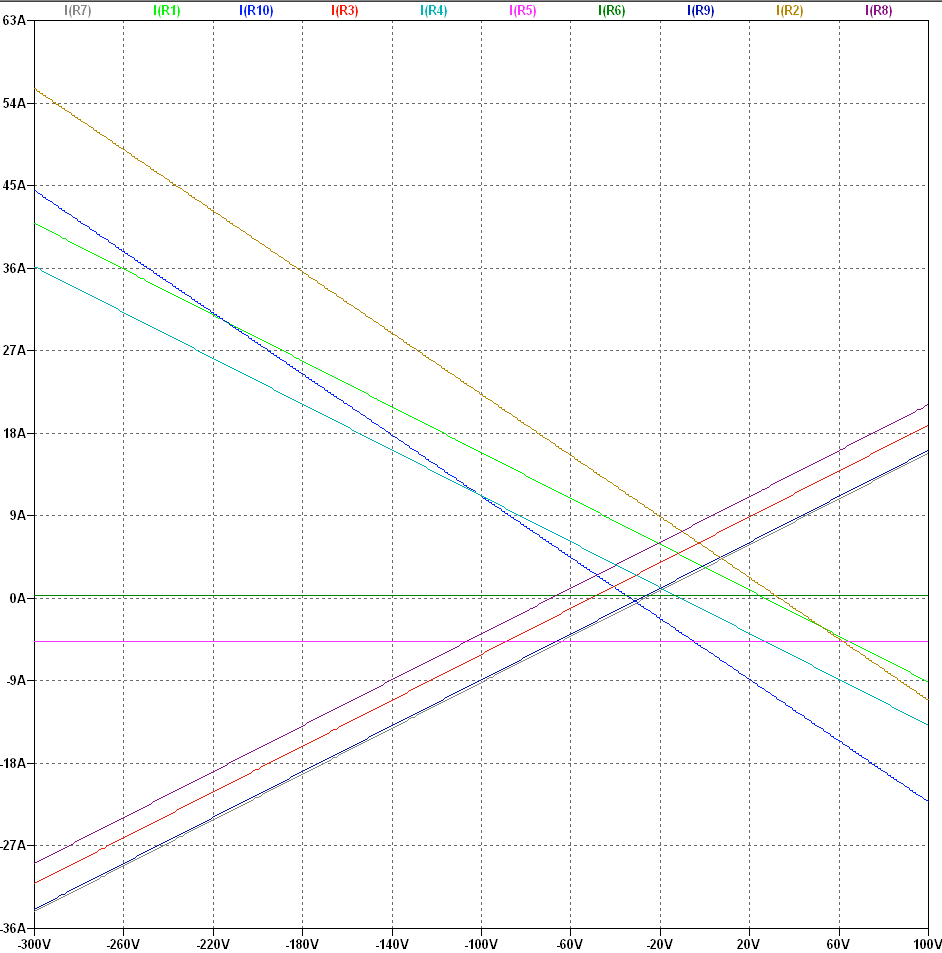
\includegraphics[width=0.8\textwidth]{./img3.png}
 \caption{Simulación usando LTSpice.}
\end{figure*}

Vemos que cuando las lineas pasan por -20 A y 20 A es donde son los ceros en nuestro programa, y los primeros cortes en esos valores, partiendo de cero, son efectivamente $\pm 86[V]$.


Acá podemos ver el gráfico con los datos de la simulación pero restándole el máximo de la corriente a 20, tal como se hizo para los métodos tanto de Cramer como PLU.

\begin{figure*}[h]
 \centering
 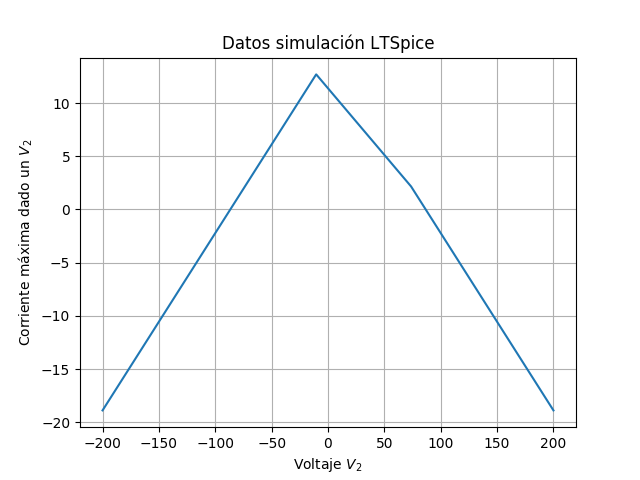
\includegraphics[width=0.8\textwidth]{./simulacion.png}
 \caption{Función objetivo con datos de simulación en LTSpice.}
\end{figure*}

Todos los archivos de las simulaciones en LTSpice también se pueden encontrar en el repositorio de la tarea.

\end{document}
